\documentclass[12pt,a4paper]{article}

\usepackage[utf8]{inputenc}
\usepackage[T1]{fontenc}
\usepackage[spanish,es-tabla]{babel}
\usepackage{lmodern}
\usepackage{geometry}
\usepackage{setspace}
\usepackage{graphicx}
\usepackage{booktabs}
\usepackage{float}
\usepackage{amsmath}
\usepackage{amssymb}
\usepackage{hyperref}
\usepackage{caption}
\usepackage{subcaption}
\usepackage{array}
\usepackage{xcolor}
\usepackage[section]{placeins}

\geometry{margin=2cm}
\graphicspath{{../outputs/figures/}}
\setstretch{1.02}
\setlength{\parindent}{0pt}
\setlength{\parskip}{0.2em}
\setlength{\floatsep}{6pt plus 1pt minus 1pt}
\setlength{\textfloatsep}{7pt plus 1pt minus 2pt}
\setlength{\intextsep}{6pt plus 1pt minus 1pt}
\setlength{\abovecaptionskip}{3pt}
\setlength{\belowcaptionskip}{0pt}
\renewcommand{\topfraction}{0.95}
\renewcommand{\bottomfraction}{0.85}
\renewcommand{\textfraction}{0.05}
\renewcommand{\floatpagefraction}{0.85}
\captionsetup{font=small,skip=3pt}
\raggedbottom
\hypersetup{
    colorlinks=true,
    linkcolor=black,
    citecolor=black,
    urlcolor=blue
}

% Archivo generado automaticamente por src/run_all.py
\newcommand{\TotalRegistros}{5224}
\newcommand{\TotalVariables}{9}
\newcommand{\FechaMinima}{2006-03-24}
\newcommand{\FechaMaxima}{2026-05-29}
\newcommand{\NulosTotales}{4}
\newcommand{\DuplicadosFecha}{0}
\newcommand{\MaxErrorProductoInverso}{0.00000000}
\newcommand{\MediaCambio}{9.2095}
\newcommand{\MedianaCambio}{8.8347}
\newcommand{\DesvioCambio}{1.5294}
\newcommand{\VarianzaCambio}{2.3389}
\newcommand{\QunoCambio}{7.8634}
\newcommand{\QtresCambio}{10.5148}
\newcommand{\IqrCambio}{2.6514}
\newcommand{\CoefVariacionCambio}{0.1661}
\newcommand{\AsimetriaCambio}{0.4673}
\newcommand{\CurtosisCambio}{-1.0273}
\newcommand{\OutliersCambio}{0}
\newcommand{\MediaLogRet}{0.000060}
\newcommand{\DesvioLogRet}{0.013001}
\newcommand{\BootstrapMediaInf}{9.1672}
\newcommand{\BootstrapMediaSup}{9.2495}
\newcommand{\CorrBrlUsdUyuUsd}{0.9819}
\newcommand{\MejorDistribucion}{lognormal}
\newcommand{\MejorDistribucionKS}{0.0763}
\newcommand{\MejorDistribucionP}{0.000000}
\newcommand{\MejorDistribucionChi}{lognormal}
\newcommand{\MejorDistribucionChiP}{0.000000}
\newcommand{\CantidadFiguras}{10}


\title{Análisis estadístico del tipo de cambio entre el peso uruguayo y el real brasileño}
\author{Fabrizio Soria \and Valentin Zamit \and Rafael Rodriguez}
\date{12/06/2026}

\begin{document}

\begin{titlepage}
    \centering
    {\Large Universidad Tecnológica del Uruguay (UTEC)\par}
    \vspace{0.12cm}
    {\large Instituto Tecnológico Regional Norte\par}
    \vspace{0.12cm}
    {\large Licenciatura en Ingeniería de Datos e Inteligencia Artificial\par}
    \vspace{1cm}
    {\Large Probabilidad y Estadística\par}
    \vspace{0.9cm}
    {\huge\bfseries Análisis estadístico del tipo de cambio entre el peso uruguayo y el real brasileño\par}
    \vspace{0.85cm}
    {\large Variable principal: cotización UYU/BRL\par}
    \vspace{0.85cm}
    \begin{tabular}{rl}
        Integrantes: & Fabrizio Soria -- CI: 56539835 \\
                     & Valentin Zamit -- CI: 56561478 \\
                     & Rafael Rodriguez -- CI: 56375401 \\
        Fuente de datos: & Yahoo Finance mediante \texttt{yfinance} \\
        Período analizado: & 24/03/2006--29/05/2026 \\
        Año: & 2026 \\
        Fecha: & 12/06/2026
    \end{tabular}
\end{titlepage}

\pagenumbering{roman}
\tableofcontents
\newpage

\section*{Resumen}
\addcontentsline{toc}{section}{Resumen}
Este trabajo analiza el comportamiento estadístico del tipo de cambio entre el peso uruguayo y el real brasileño, expresado como la cantidad de pesos uruguayos necesarios para adquirir un real brasileño. El estudio sigue el recorrido metodológico trabajado en el curso: definición de población y muestra, análisis exploratorio, modelización probabilística e inferencia estadística. El fenómeno resulta relevante por la relación económica, comercial y turística entre Uruguay y Brasil. Se utilizó un conjunto de datos históricos obtenido desde Yahoo Finance mediante Python, construido a partir de las cotizaciones del dólar frente al peso uruguayo y frente al real brasileño. La muestra contiene \TotalRegistros{} observaciones correspondientes al período \FechaMinima{} a \FechaMaxima{}.

La variable principal del estudio es \texttt{uyu\_por\_brl}. Se aplicaron medidas de tendencia central, cuartiles, IQR, varianza y desvío estándar; además, se utilizaron histogramas, boxplots, Q-Q plots, autocorrelación, ajuste de distribuciones e intervalos de confianza. Los resultados iniciales muestran una media muestral de \MediaCambio{} UYU/BRL, una mediana de \MedianaCambio{} y una dispersión muestral de \DesvioCambio{}. La distribución con mejor ajuste relativo fue la \MejorDistribucionChi{}, seguida por la \SegundaDistribucionChi{}, aunque la prueba chi-cuadrado rechazó todos los modelos evaluados al 5\%. La evidencia indica estructura temporal, por lo que la inferencia clásica debe interpretarse con cautela.

\textbf{Palabras clave:} tipo de cambio, UYU/BRL, serie temporal, inferencia estadística, autocorrelación.

\newpage
\pagenumbering{arabic}

\section{Introducción}

El curso de Probabilidad y Estadística organiza el trabajo estadístico como un proceso que parte de la identificación del fenómeno, continúa con la recolección y exploración de datos, y culmina con una etapa de inferencia apoyada en modelos probabilísticos \cite{curso_intro}. En este marco, el presente informe analiza el tipo de cambio entre el peso uruguayo y el real brasileño, expresado como la cantidad de pesos uruguayos necesarios para comprar un real brasileño.

El fenómeno resulta relevante para Uruguay por la cercanía económica y regional con Brasil. Las variaciones del real frente al peso pueden incidir en decisiones vinculadas al turismo, al comercio, a compras transfronterizas y a la comparación de precios entre ambos países. Desde el punto de vista estadístico, se trata de una variable cuantitativa continua observada en el tiempo, por lo que permite aplicar herramientas de análisis exploratorio, distribución empírica, modelización probabilística, intervalos de confianza y análisis de autocorrelación.

La variable principal es \texttt{uyu\_por\_brl}. Si se denota por \(X_t\) la cotización diaria UYU/BRL en el instante \(t\), cada observación representa el valor de esa variable en una fecha para la cual existen simultáneamente las cotizaciones necesarias. La pregunta principal del trabajo es: \textit{¿cuál es el comportamiento estadístico del tipo de cambio entre el peso uruguayo y el real brasileño durante el período analizado, y qué características presentan su distribución, variabilidad y dependencia temporal?}

El objetivo general es analizar estadísticamente el comportamiento del tipo de cambio entre el peso uruguayo y el real brasileño, evaluando su distribución empírica, su posible modelado probabilístico, su evolución temporal y la incertidumbre asociada a sus principales parámetros.

Los objetivos específicos son:

\begin{itemize}
    \item describir la cotización UYU/BRL mediante medidas de tendencia central, dispersión y posición, junto con histogramas y boxplots;
    \item analizar el comportamiento temporal de la cotización mediante gráficos, diagramas con rezagos y autocorrelaciones;
    \item evaluar qué distribución teórica se ajusta mejor a los datos usando histogramas, Q-Q plots y prueba chi-cuadrado de bondad de ajuste;
    \item construir e interpretar intervalos de confianza para la media y la varianza, considerando distintos niveles de confianza y los supuestos necesarios.
\end{itemize}

El informe se estructura en ocho secciones. Luego de la introducción se presenta la metodología de construcción y preparación de datos. Después se desarrolla el análisis descriptivo, el análisis temporal, la evaluación de distribuciones teóricas, los intervalos de confianza, la discusión y las conclusiones.


\section{Metodología}

La fuente de datos utilizada fue Yahoo Finance, accedida mediante la librería \texttt{yfinance} de Python. Como no se trabajó con una cotización directa UYU/BRL, se descargaron dos series cambiarias: \texttt{USDUYU=X}, que representa pesos uruguayos por dólar estadounidense, y \texttt{USDBRL=X}, que representa reales brasileños por dólar estadounidense. A partir de ambas series se construyó la variable principal:

\[
    \text{UYU/BRL} = \frac{\text{UYU/USD}}{\text{BRL/USD}}.
\]

La unidad estadística corresponde a una observación diaria con datos completos para ambas cotizaciones. La población de interés se interpreta como el conjunto de valores posibles del tipo de cambio UYU/BRL durante el período de estudio. La muestra efectiva contiene \TotalRegistros{} registros entre \FechaMinima{} y \FechaMaxima{}.

El archivo original contiene siete columnas: fecha, cotizaciones base frente al dólar, cotización directa construida UYU/BRL, cotización inversa BRL/UYU, retorno diario y log-retorno de la cotización inversa. Durante el procesamiento reproducible se agregaron dos variables derivadas para la cotización principal: \texttt{retorno\_diario\_uyu\_por\_brl} y \texttt{log\_retorno\_uyu\_por\_brl}; por eso las tablas generadas informan \TotalVariables{} variables. Se validó la presencia de las columnas esperadas, se ordenaron las observaciones por fecha y se calcularon valores faltantes. El total de nulos detectado luego de crear retornos fue \NulosTotales{}, correspondientes al primer valor no definido de las series de retornos. No se detectaron fechas duplicadas: \DuplicadosFecha{}.

También se verificó la relación recíproca entre \texttt{uyu\_por\_brl} y \texttt{brl\_por\_uyu}. El máximo error absoluto observado en el producto \(\text{UYU/BRL}\times\text{BRL/UYU}\) fue \MaxErrorProductoInverso{}, lo que confirma que ambas columnas representan la misma relación cambiaria en sentidos inversos.

El análisis se realizó con Python, usando principalmente \texttt{pandas}, \texttt{numpy}, \texttt{matplotlib}, \texttt{seaborn}, \texttt{scipy} y \texttt{statsmodels}. El informe se redactó en LaTeX. La metodología estadística incluyó:

\begin{itemize}
    \item medidas descriptivas de la cotización UYU/BRL y de los log-retornos;
    \item histogramas, boxplots, Q-Q plots y gráficos de evolución temporal;
    \item autocorrelación de log-retornos para diferentes rezagos;
    \item correlaciones de Pearson entre variables cambiarias;
    \item comparación de distribuciones Normal, Log-normal y Gamma mediante prueba Kolmogorov-Smirnov;
    \item intervalos de confianza clásicos para media y varianza, y un intervalo bootstrap para la media.
\end{itemize}

Una limitación metodológica importante es que la muestra no surge de un muestreo aleatorio simple, sino de una serie histórica observacional. Por lo tanto, la independencia entre observaciones no puede asumirse automáticamente. Además, al tratarse de datos financieros, los resultados deben interpretarse como evidencia descriptiva e inferencial condicionada al período observado, no como una afirmación causal.

\section{Análisis descriptivo}

El análisis exploratorio de datos permite describir la distribución empírica antes de proponer un modelo probabilístico. En los materiales del curso se enfatiza que cuartiles, IQR, boxplot e histograma permiten estudiar concentración, variabilidad y valores atípicos \cite{curso_eda}. La Tabla \ref{tab:resumen-descriptivo} resume las medidas principales de \texttt{uyu\_por\_brl}; las tablas completas quedan disponibles en \texttt{outputs/tables/}.

\begin{table}[htbp]
\centering
\small
\caption{Resumen descriptivo de la cotización UYU/BRL.}
\label{tab:resumen-descriptivo}
\begin{tabular}{lr@{\hspace{1cm}}lr}
\toprule
Medida & Valor & Medida & Valor \\
\midrule
Media & \MediaCambio{} & Mediana & \MedianaCambio{} \\
Desvío estándar & \DesvioCambio{} & Varianza & \VarianzaCambio{} \\
Q1 & \QunoCambio{} & Q3 & \QtresCambio{} \\
IQR & \IqrCambio{} & Outliers IQR & \OutliersCambio{} \\
Coef. variación & \CoefVariacionCambio{} & Asimetría & \AsimetriaCambio{} \\
\bottomrule
\end{tabular}
\end{table}

La media resume el centro de la distribución, pero no describe por sí sola la variabilidad; por eso se complementa con varianza y desvío estándar, siguiendo el enfoque del curso sobre media y varianza \cite{curso_media_varianza}. El criterio de \(1.5IQR\) no detectó valores atípicos, aunque esto no elimina la presencia de cambios temporales relevantes.

\begin{figure}[htbp]
    \centering
    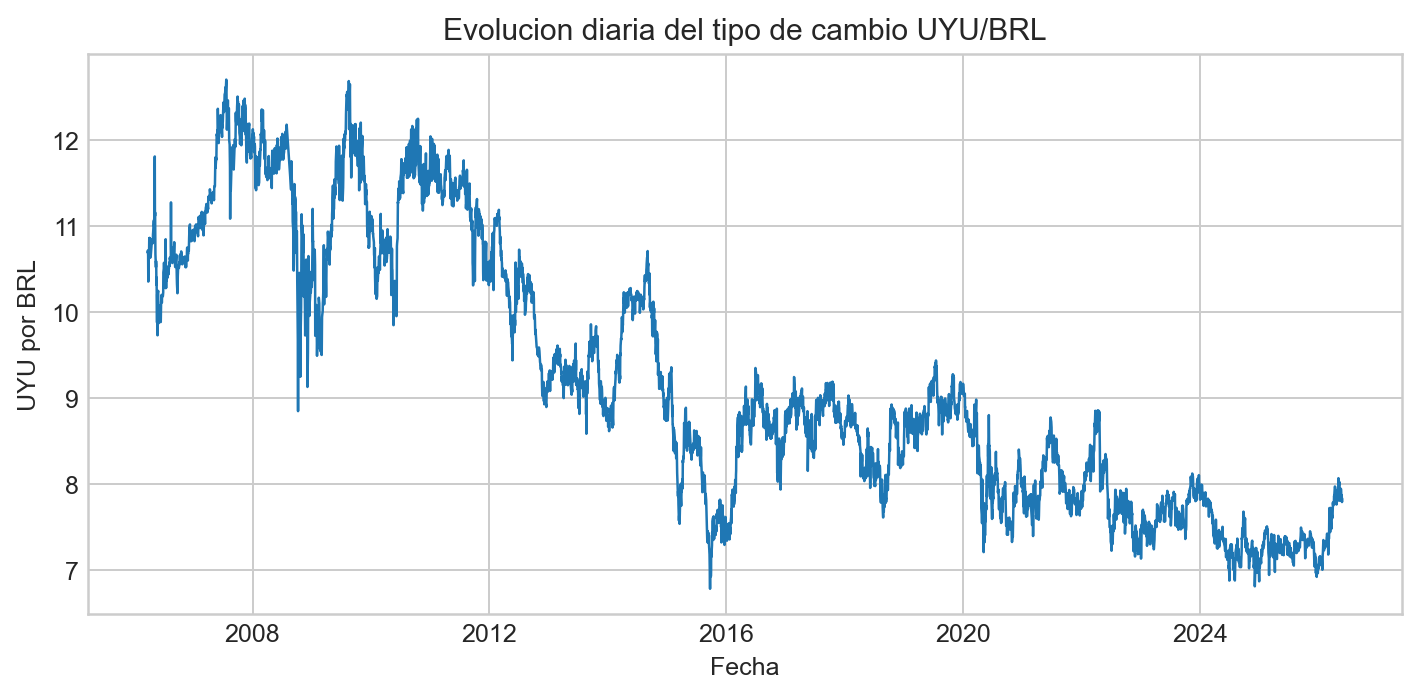
\includegraphics[width=0.82\textwidth]{serie_uyu_por_brl.png}
    \caption{Evolución temporal diaria de la cotización expresada en pesos uruguayos por real brasileño. Fuente: elaboración propia a partir de Yahoo Finance.}
    \label{fig:serie-cambio}
\end{figure}

La Figura \ref{fig:serie-cambio} evidencia que la cotización no se comporta como una colección de observaciones sin orden. Existen períodos de suba, baja y cambios de nivel. Esta estructura temporal es central: antes de aplicar inferencia clásica, debe considerarse que observaciones próximas en el tiempo pueden estar relacionadas.

\begin{figure}[htbp]
    \centering
    \begin{subfigure}{0.47\textwidth}
        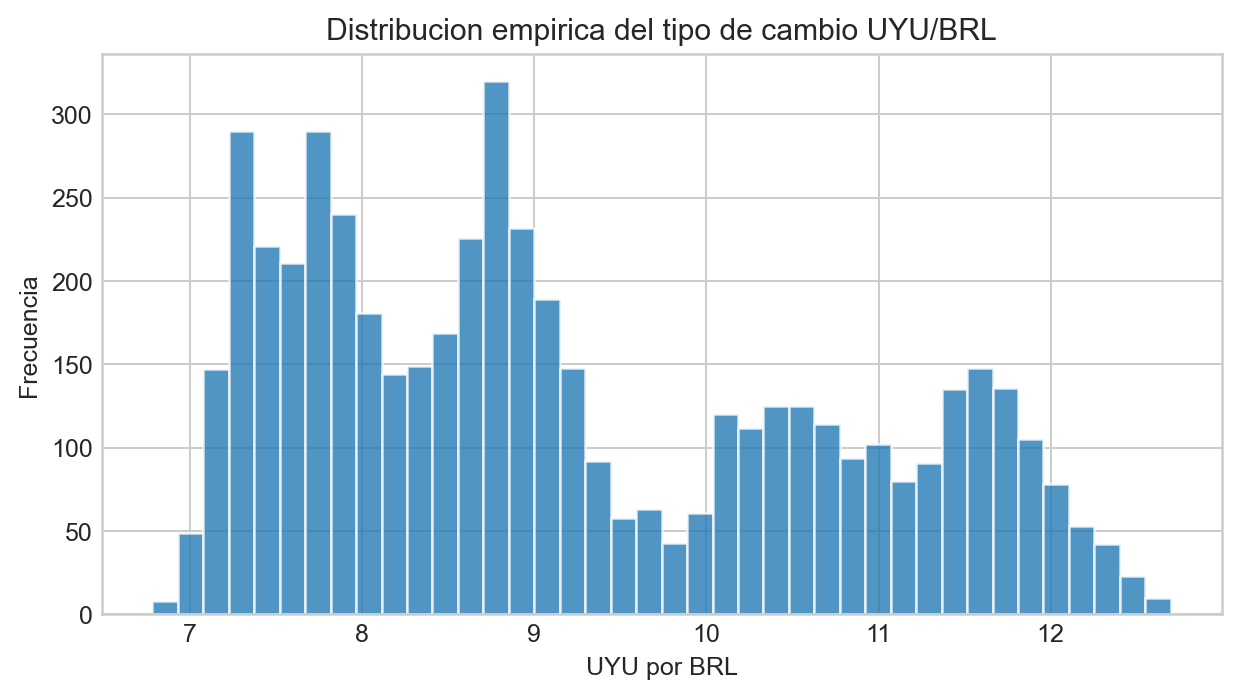
\includegraphics[width=\textwidth]{hist_uyu_por_brl.png}
        \caption{Histograma}
        \label{fig:hist-cambio}
    \end{subfigure}
    \hfill
    \begin{subfigure}{0.47\textwidth}
        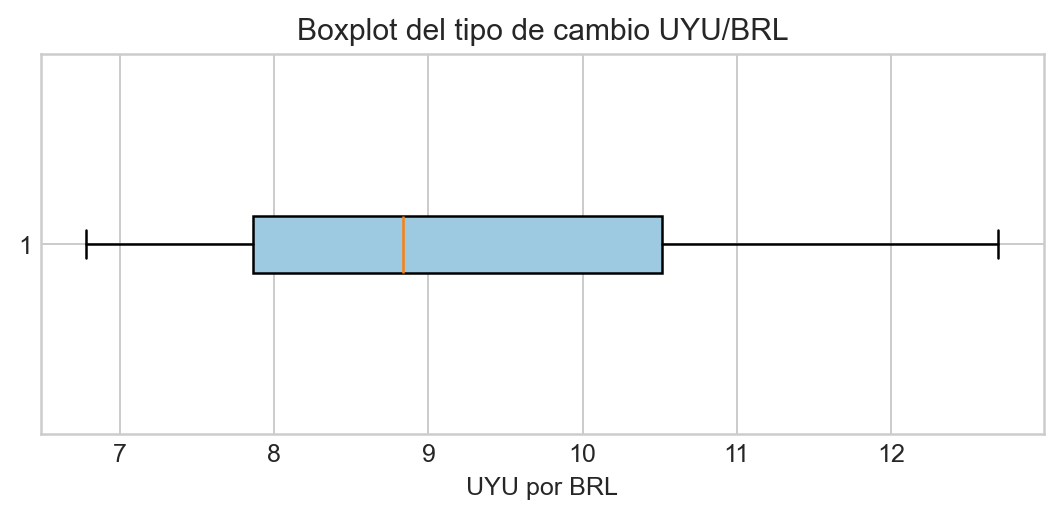
\includegraphics[width=\textwidth]{boxplot_uyu_por_brl.png}
        \caption{Boxplot}
        \label{fig:box-cambio}
    \end{subfigure}
    \caption{Distribución empírica y resumen gráfico de la cotización UYU/BRL. Fuente: elaboración propia a partir de Yahoo Finance.}
    \label{fig:dist-box}
\end{figure}

El histograma de la Figura \ref{fig:dist-box} muestra la distribución de frecuencias por clases, tal como se trabaja en el curso para aproximar visualmente la distribución empírica. El boxplot resume mediana, cuartiles y dispersión central. La revisión de retornos y volatilidad se conserva en los archivos generados, pero no se inserta como figura adicional para evitar redundancias en el informe.

\section{Distribución teórica}

La distribución empírica de \texttt{uyu\_por\_brl} se comparó con distribuciones teóricas continuas. Como primera aproximación se consideraron las distribuciones Normal, Log-normal y Gamma, porque son candidatas usuales para variables continuas positivas o aproximadamente simétricas. La comparación se realizó mediante la prueba Kolmogorov-Smirnov, ajustando previamente los parámetros de cada distribución candidata.

\begin{figure}[H]
    \centering
    \begin{subfigure}{0.48\textwidth}
        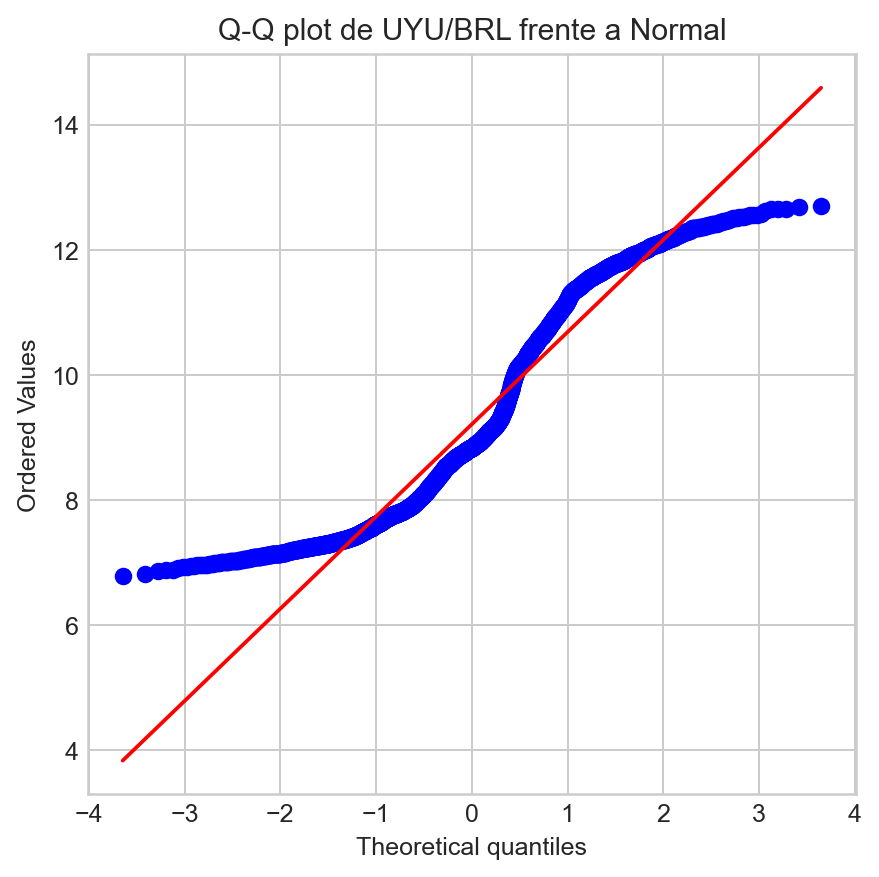
\includegraphics[width=\textwidth]{qq_uyu_por_brl.png}
        \caption{Cotización UYU/BRL}
        \label{fig:qq-cambio}
    \end{subfigure}
    \hfill
    \begin{subfigure}{0.48\textwidth}
        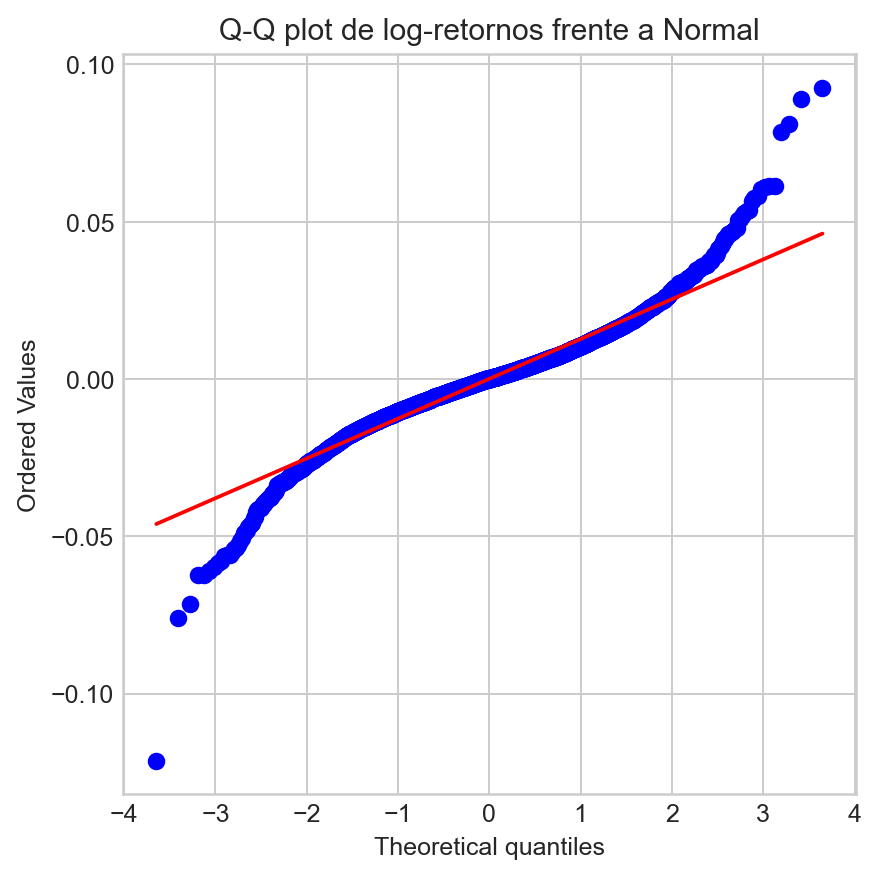
\includegraphics[width=\textwidth]{qq_log_retornos.png}
        \caption{Log-retornos}
        \label{fig:qq-retornos}
    \end{subfigure}
    \caption{Q-Q plots frente a la distribución Normal.}
    \label{fig:qqplots}
\end{figure}

El Q-Q plot de la cotización permite evaluar visualmente si los cuantiles observados se alinean con los cuantiles esperados bajo normalidad. En series financieras, los retornos suelen ser más adecuados para estudiar supuestos distribucionales que los niveles de la cotización, porque estos últimos pueden presentar tendencia, cambios de régimen y dependencia temporal.

\begin{table}[H]
\centering
\small
\caption{Comparacion de distribuciones candidatas mediante prueba KS.}
\label{tab:bondad-ajuste}
\resizebox{\textwidth}{!}{%
\begin{tabular}{llll}
\toprule
distribucion & parametros & ks\_estadistico & p\_value \\
\midrule
lognormal & 0.162769; 0; 9.08678 & 0.0763 & 0.0000 \\
gamma & 37.4396; 0; 0.245983 & 0.0866 & 0.0000 \\
normal & 9.2095; 1.52921 & 0.1064 & 0.0000 \\
\bottomrule
\end{tabular}%
}
\end{table}


\begin{table}[H]
\centering
\small
\caption{Comparacion de distribuciones candidatas mediante prueba chi-cuadrado.}
\label{tab:bondad-ajuste-chi2}
\resizebox{\textwidth}{!}{%
\begin{tabular}{llllllll}
\toprule
distribucion & clases & parametros\_estimados & frecuencia\_esperada\_minima & grados\_libertad & chi2\_estadistico & p\_value & decision\_alpha\_0\_05 \\
\midrule
Log-normal & 12 & 3 & 435.3333 & 8 & 1064.4594 & 0.0000 & Se rechaza H0 \\
Gamma & 12 & 3 & 435.3333 & 8 & 1324.7519 & 0.0000 & Se rechaza H0 \\
Normal & 12 & 2 & 435.3333 & 9 & 1817.2343 & 0.0000 & Se rechaza H0 \\
\bottomrule
\end{tabular}%
}
\end{table}


Según el criterio KS, la mejor distribución entre las candidatas evaluadas fue \MejorDistribucion{}, con estadístico \MejorDistribucionKS{} y p-value \MejorDistribucionP{}. La prueba chi-cuadrado también ubicó a \MejorDistribucionChi{} como el ajuste relativo más favorable entre las alternativas comparadas, aunque con p-value \MejorDistribucionChiP{}. En consecuencia, la evidencia disponible no permite afirmar que la distribución sea exacta; solamente permite señalar qué candidata se comportó relativamente mejor bajo los criterios utilizados.

\begin{figure}[H]
    \centering
    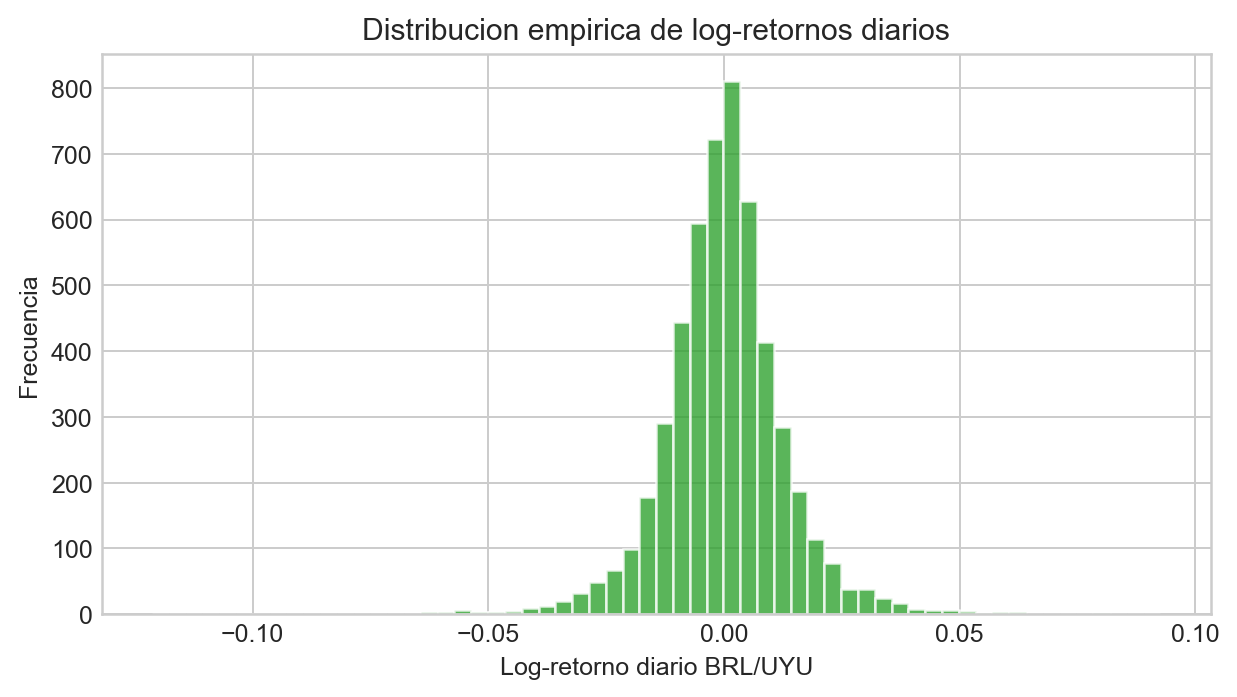
\includegraphics[width=0.80\textwidth]{hist_log_retornos.png}
    \caption{Distribución empírica de los log-retornos diarios.}
    \label{fig:hist-retornos}
\end{figure}

El análisis de log-retornos complementa el estudio de la cotización en niveles, ya que permite observar las variaciones relativas diarias. Esta transformación es habitual en datos financieros y ayuda a evaluar la estabilidad de la serie, aunque no garantiza por sí misma normalidad ni independencia.

\section{Intervalos de confianza}

La inferencia estadística busca usar información muestral para aproximar parámetros poblacionales. En el curso, este paso se apoya en distribuciones muestrales de estadísticos como la media, la varianza, la distribución t-Student y la distribución chi-cuadrado \cite{curso_muestreo}. En este trabajo se estimaron intervalos para la media y la varianza de \texttt{uyu\_por\_brl}.

Para la media, con varianza poblacional desconocida, se utilizó el intervalo basado en t-Student:

\[
    \bar{x} \pm t_{\alpha/2,n-1}\frac{s}{\sqrt{n}},
\]

donde \(\bar{x}\) es la media muestral, \(s\) el desvío estándar muestral y \(n\) el tamaño de muestra.

\begin{table}[H]
\centering
\small
\caption{Intervalos de confianza clasicos para la media de UYU/BRL.}
\label{tab:ic-media-cambio}
\resizebox{\textwidth}{!}{%
\begin{tabular}{llllll}
\toprule
nivel\_confianza & media & limite\_inferior & limite\_superior & amplitud & metodo \\
\midrule
0.9000 & 9.2095 & 9.1747 & 9.2443 & 0.0696 & t de Student \\
0.9500 & 9.2095 & 9.1680 & 9.2510 & 0.0830 & t de Student \\
0.9900 & 9.2095 & 9.1550 & 9.2640 & 0.1090 & t de Student \\
\bottomrule
\end{tabular}%
}
\end{table}


Para la varianza, bajo supuesto de normalidad e independencia, se utiliza la distribución chi-cuadrado:

\[
    \left(
    \frac{(n-1)s^2}{\chi^2_{1-\alpha/2,n-1}},
    \frac{(n-1)s^2}{\chi^2_{\alpha/2,n-1}}
    \right).
\]

\begin{table}[H]
\centering
\small
\caption{Intervalos de confianza clasicos para la varianza de UYU/BRL.}
\label{tab:ic-varianza-cambio}
\resizebox{\textwidth}{!}{%
\begin{tabular}{llllll}
\toprule
nivel\_confianza & varianza\_muestral & limite\_inferior & limite\_superior & amplitud & metodo \\
\midrule
0.9000 & 2.3389 & 2.2655 & 2.4162 & 0.1506 & chi-cuadrado \\
0.9500 & 2.3389 & 2.2517 & 2.4313 & 0.1795 & chi-cuadrado \\
0.9900 & 2.3389 & 2.2252 & 2.4612 & 0.2360 & chi-cuadrado \\
\bottomrule
\end{tabular}%
}
\end{table}


Al aumentar el nivel de confianza, aumenta la amplitud del intervalo. Esto ocurre porque el procedimiento exige un rango más amplio de valores compatibles con el parámetro. La interpretación correcta no es que exista una probabilidad del 95\% de que el parámetro fijo esté dentro del intervalo ya calculado, sino que el método produce intervalos que, en repeticiones del muestreo bajo sus supuestos, cubren el parámetro con esa frecuencia aproximada.

También se calculó un intervalo bootstrap percentil al 95\% para la media: [\BootstrapMediaInf{}; \BootstrapMediaSup{}]. El bootstrap aporta una alternativa empírica, pero en series temporales el remuestreo simple puede romper la dependencia entre observaciones. Por este motivo, una extensión metodológica más adecuada sería implementar bootstrap por bloques.


\section{Pruebas de hipótesis}

Las pruebas de hipótesis se aplicaron para evaluar normalidad, asociación lineal y dependencia temporal. En todos los casos se consideró un nivel de significancia de referencia \(\alpha = 0.05\), sin perder de vista que la significancia estadística no implica importancia práctica ni causalidad.

\subsection{Normalidad}

Para la cotización UYU/BRL y los log-retornos se planteó:

\[
    H_0: \text{los datos provienen de una distribución Normal}
\]
\[
    H_1: \text{los datos no provienen de una distribución Normal}.
\]

\begin{table}[H]
\centering
\small
\caption{Pruebas de normalidad para la cotizacion y los log-retornos.}
\label{tab:normalidad}
\resizebox{\textwidth}{!}{%
\begin{tabular}{llll}
\toprule
variable & prueba & estadistico & p\_value \\
\midrule
uyu\_por\_brl & D'Agostino-Pearson & 1547.5193 & 0.0000 \\
uyu\_por\_brl & Kolmogorov-Smirnov estandarizado & 0.1064 & 0.0000 \\
log\_retorno\_brl\_por\_uyu & D'Agostino-Pearson & 617.6060 & 0.0000 \\
log\_retorno\_brl\_por\_uyu & Kolmogorov-Smirnov estandarizado & 0.0624 & 0.0000 \\
\bottomrule
\end{tabular}%
}
\end{table}


Si el p-value es menor que 0.05, se rechaza la hipótesis nula de normalidad. En muestras grandes, este rechazo puede ocurrir aun cuando las desviaciones visuales sean moderadas, por lo que se complementa la interpretación con histogramas y Q-Q plots.

\subsection{Correlaciones entre variables cambiarias}

Se evaluaron correlaciones de Pearson entre las variables numéricas principales. Para cada par se planteó:

\[
    H_0: \rho = 0
\]
\[
    H_1: \rho \neq 0.
\]

\begin{table}[H]
\centering
\small
\caption{Correlaciones de Pearson entre variables cambiarias.}
\label{tab:correlaciones}
\resizebox{\textwidth}{!}{%
\begin{tabular}{lllll}
\toprule
variable\_x & variable\_y & pearson\_r & p\_value & n \\
\midrule
brl\_por\_usd & uyu\_por\_usd & 0.9819 & 0.0000 & 5224 \\
brl\_por\_usd & uyu\_por\_brl & -0.8885 & 0.0000 & 5224 \\
uyu\_por\_usd & uyu\_por\_brl & -0.8102 & 0.0000 & 5224 \\
brl\_por\_uyu & uyu\_por\_brl & -0.9899 & 0.0000 & 5224 \\
\bottomrule
\end{tabular}%
}
\end{table}


La correlación entre \texttt{brl\_por\_usd} y \texttt{uyu\_por\_usd} fue \CorrBrlUsdUyuUsd{}. Este resultado indica asociación lineal en el período observado, pero no permite afirmar causalidad entre ambas series. Ambas variables pueden responder simultáneamente a factores macroeconómicos, monetarios y financieros externos.

\begin{figure}[H]
    \centering
    \begin{subfigure}{0.48\textwidth}
        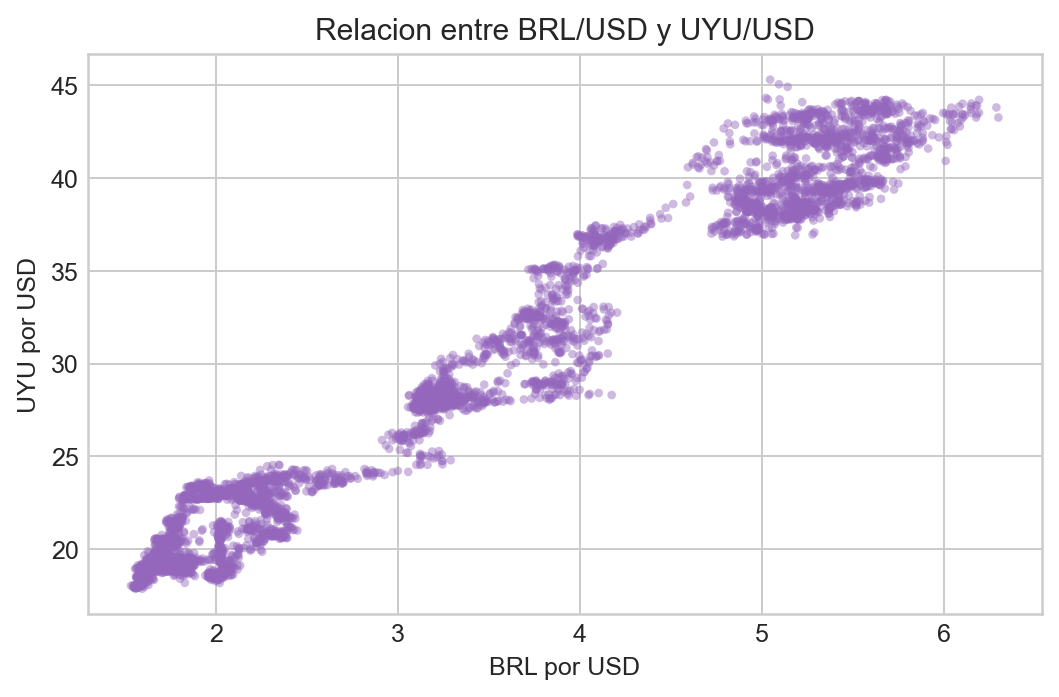
\includegraphics[width=\textwidth]{scatter_brl_usd_vs_uyu_usd.png}
        \caption{Dispersión BRL/USD vs UYU/USD}
        \label{fig:scatter}
    \end{subfigure}
    \hfill
    \begin{subfigure}{0.48\textwidth}
        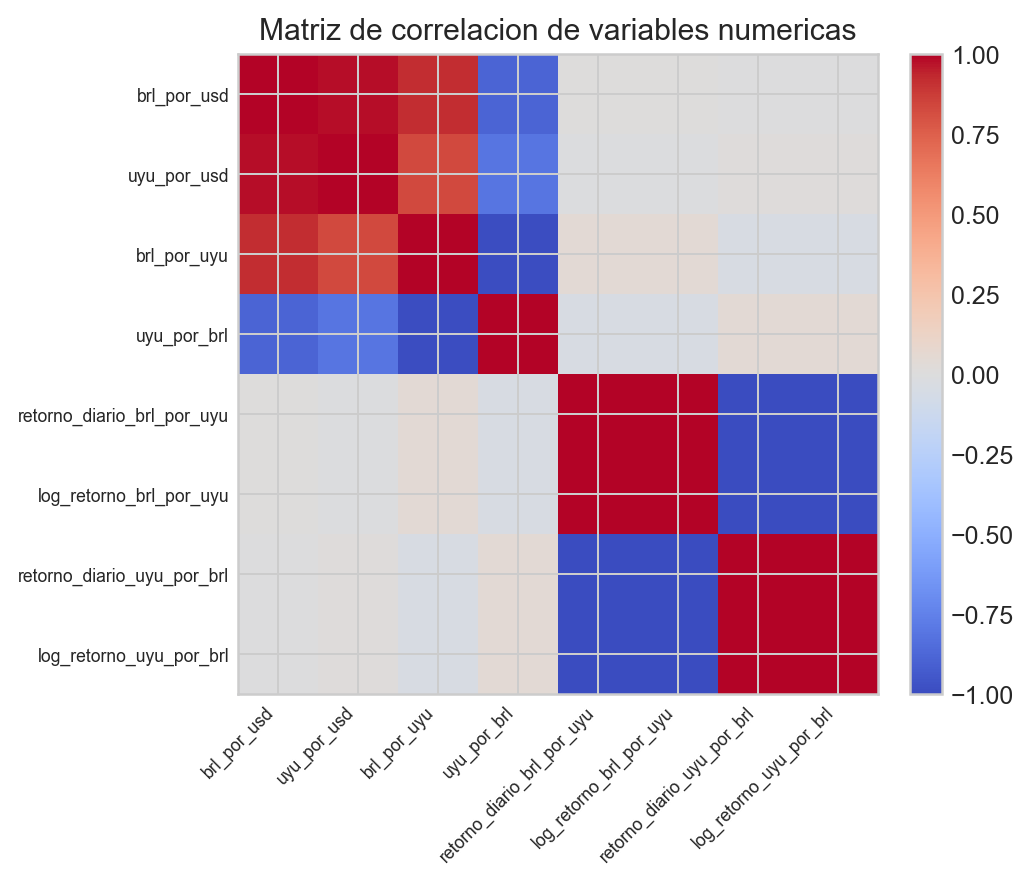
\includegraphics[width=\textwidth]{matriz_correlacion.png}
        \caption{Matriz de correlación}
        \label{fig:heatmap}
    \end{subfigure}
    \caption{Relaciones lineales entre variables cambiarias.}
    \label{fig:correlaciones}
\end{figure}

\subsection{Autocorrelación de retornos}

Para estudiar dependencia temporal en los log-retornos se calculó la autocorrelación para distintos rezagos. Conceptualmente, se contrasta si la correlación entre la serie y sus valores rezagados es nula.

\begin{table}[H]
\centering
\small
\caption{Autocorrelacion de log-retornos para los primeros rezagos.}
\label{tab:autocorrelacion}
\resizebox{\textwidth}{!}{%
\begin{tabular}{ll}
\toprule
lag & autocorrelacion \\
\midrule
0 & 1.0000 \\
1 & -0.1917 \\
2 & -0.0571 \\
3 & -0.0264 \\
4 & -0.0159 \\
5 & -0.0091 \\
6 & -0.0128 \\
7 & 0.0234 \\
8 & 0.0181 \\
9 & -0.0434 \\
10 & 0.0588 \\
\bottomrule
\end{tabular}%
}
\end{table}


\begin{figure}[H]
    \centering
    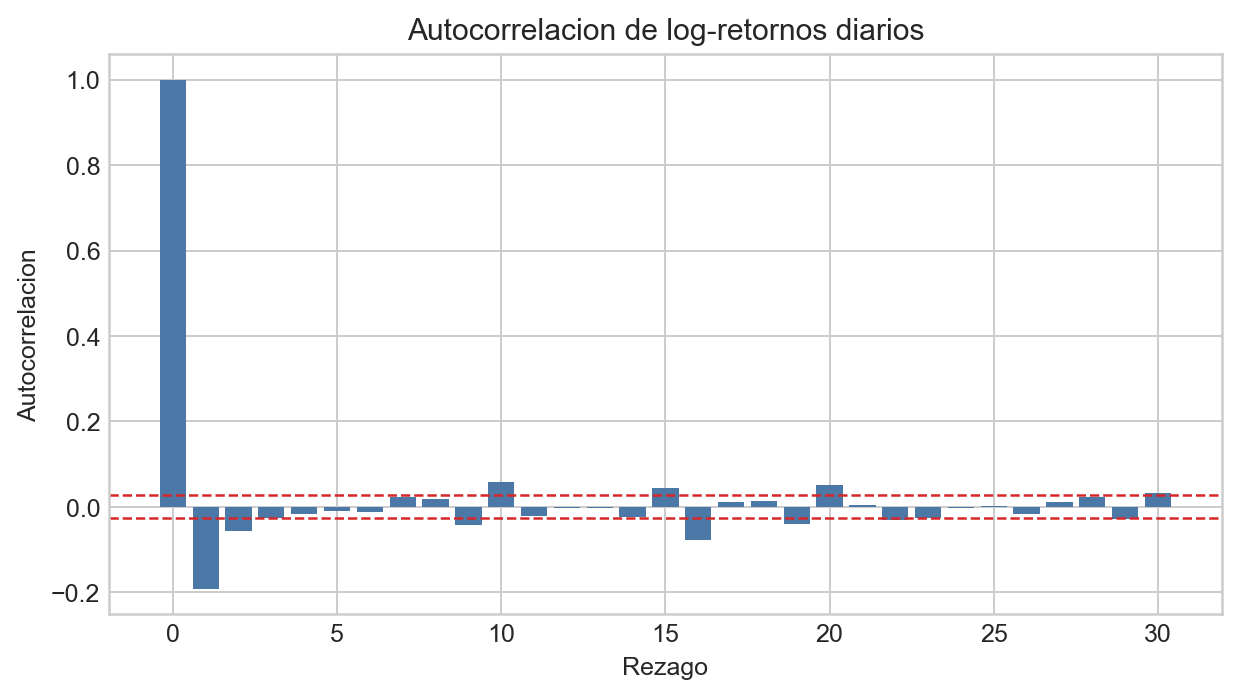
\includegraphics[width=0.80\textwidth]{acf_log_retornos.png}
    \caption{Autocorrelación de log-retornos diarios para distintos rezagos.}
    \label{fig:acf}
\end{figure}

La presencia de autocorrelaciones relevantes indicaría que las observaciones no son completamente independientes. Esta característica es importante porque varios procedimientos inferenciales clásicos suponen independencia muestral. Como no se implementó una prueba Ljung-Box en esta versión, queda como mejora posible para una revisión posterior.

\section{Discusión}

Los resultados muestran que el tipo de cambio UYU/BRL presenta variación apreciable durante el período estudiado. La media muestral de \MediaCambio{} y el desvío estándar de \DesvioCambio{} ofrecen una primera síntesis del comportamiento central y de la dispersión, pero la serie temporal evidencia cambios de nivel y períodos de distinta volatilidad.

El análisis gráfico indica que la distribución empírica de la cotización no debe interpretarse aisladamente de su evolución temporal. Una cotización financiera observada durante muchos años puede mezclar distintos contextos económicos, por lo que una única distribución teórica puede ser útil como aproximación descriptiva, pero no necesariamente como modelo completo del fenómeno.

Los log-retornos ayudan a estudiar las variaciones diarias de forma más estable. Aun así, la normalidad no puede asumirse sin revisión, y la autocorrelación debe considerarse al interpretar intervalos y pruebas. En este sentido, los métodos clásicos son didácticamente útiles y permiten aplicar herramientas del curso, pero deben complementarse con enfoques empíricos o específicos de series temporales cuando se busca mayor rigurosidad.

Una limitación importante es que los datos no provienen de un muestreo aleatorio simple. Se trata de observaciones históricas disponibles, condicionadas por días de mercado, disponibilidad de cotizaciones y el procedimiento de construcción indirecta de UYU/BRL. Además, las asociaciones entre variables cambiarias no implican causalidad: pueden existir factores externos comunes que afecten simultáneamente al peso uruguayo, al real brasileño y al dólar estadounidense.


\section{Conclusiones}

El trabajo permitió analizar el tipo de cambio UYU/BRL como una variable cuantitativa continua observada en el tiempo. La muestra contiene \TotalRegistros{} registros entre \FechaMinima{} y \FechaMaxima{}. La media muestral fue \MediaCambio{}, la mediana fue \MedianaCambio{} y el desvío estándar fue \DesvioCambio{}, lo que resume el nivel central y la variabilidad de la cotización en el período estudiado.

La distribución empírica fue explorada mediante histograma, boxplot, cuartiles e IQR. No se detectaron outliers por el criterio de 1.5 IQR, pero sí se observaron cambios de nivel y variabilidad temporal. Por ello, la variable no debe tratarse como una muestra independiente sin estructura temporal.

Entre las distribuciones candidatas evaluadas para el nivel de la cotización, la Log-normal presentó el mejor ajuste relativo según KS y chi-cuadrado. Sin embargo, la evidencia no permite afirmar que esa distribución describa exactamente el fenómeno real. El ajuste debe interpretarse como una aproximación útil, no como una verdad probabilística definitiva.

Los intervalos de confianza para la media y la varianza aplican herramientas centrales del curso, pero su interpretación debe considerar la dependencia temporal. Para mejorar el análisis se recomienda incorporar pruebas de autocorrelación conjunta, bootstrap por bloques, modelos específicos de series temporales, análisis por subperíodos y comparación con otras fuentes de datos.

En síntesis, el análisis describe el comportamiento observado del tipo de cambio UYU/BRL, cuantifica su variabilidad y evalúa modelos probabilísticos posibles. Su utilidad principal es organizar evidencia estadística sobre el período estudiado, no producir una predicción cierta ni establecer relaciones causales.



\nocite{actividad_final_pye}
\bibliographystyle{plain}
\bibliography{references}

\end{document}
